\subsection{\ltwotau channel}{\Large\bfseries}
\label{sec:1l2taus}

The \ltwotau channel is primarily sensitive to \hhtowwtt decay mode and about $80\%$ of signal events come from this mode, as shown in Figure~\ref{fig:HHdmode}. In such decay mode, one of the W boson decays into a lepton and neutrino while other to hadrons. The tau leptons decay hadronically. A signal event is expected to be characterized by the presence of one light lepton, two hadronically decaying $\tau$ leptons, missing energy from neutrinos and lower jet multiplicity. At lest two reconstructed jets are expected in such events, not taking into account the additional jets from initial and final state radiation.

\begin{figure}[hbtp]
  \begin{center}
    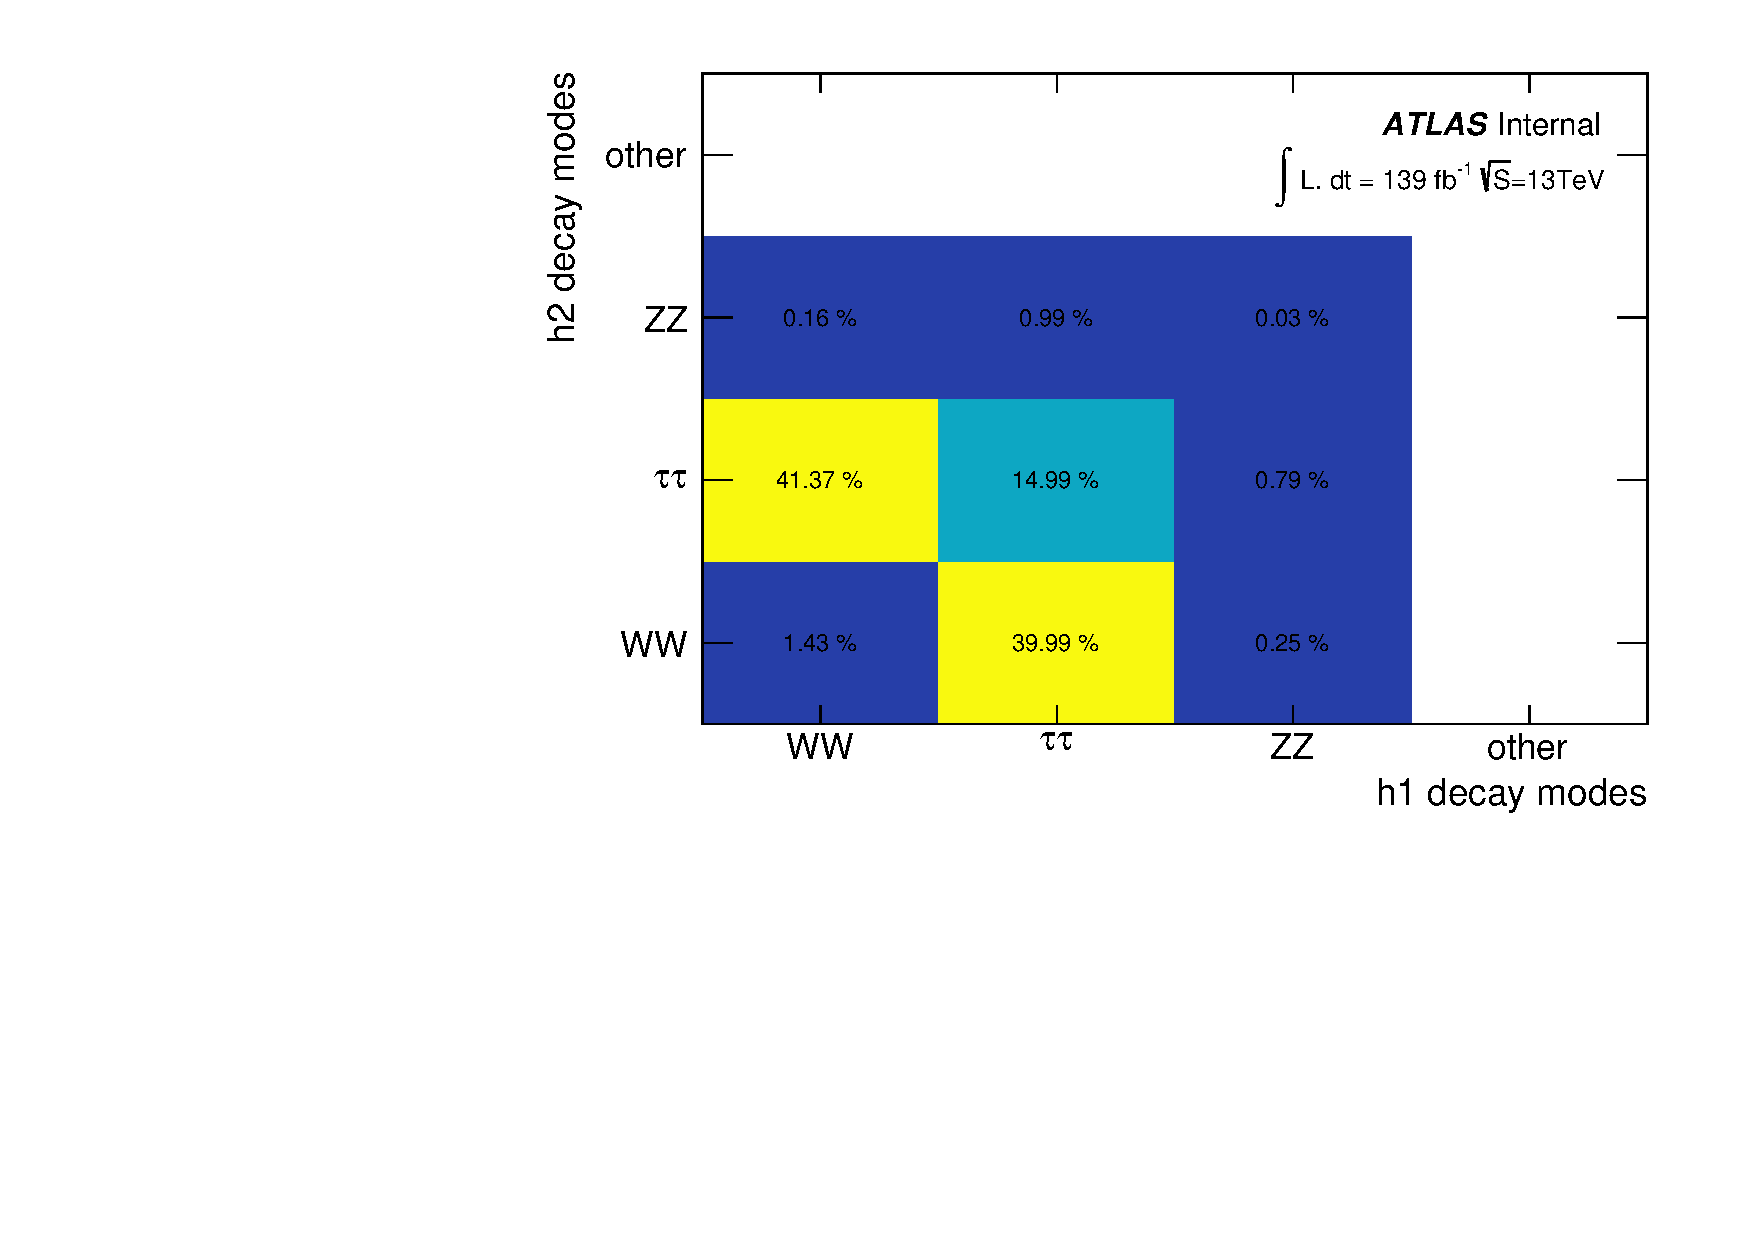
\includegraphics[width=0.7\textwidth]{figures/TauChannels/1l2tau/HHDecayModes}
    \caption{\label{fig:HHdmode} DiHiggs decay modes in the \ltwotau channel.}
  \end{center}
\end{figure}


\subsubsection{Event selection}
Events are selected by requiring exactly one light lepton (electron or muon) and exactly two hadronically decaying $\tau$ leptons. The lepton is required to pass \textit{loose} selection as described in Section~\ref{sec:objselec}, and summarized in Table~\ref{tab:objdef_1lep}. The \tauh candidates are required to pass the selection of Table~\ref{tab:taudef_2taus} and must be of opposite charge. In this channel, a single lepton trigger (Table~\ref{tab:triggers_mb2}) is used to select the events. The light lepton is required to be matched to the trigger signature. Events must have at least two reconstructed jets. A veto on events containing $b$ jets, corresponds to working point with an average efficiecny of $77\%$, is applied. In order to suppress the \vjet background, the angular distance between the two \tauh candidates is required to be less than 2. The event selection is based on the signal region optimisation study presented in Section~\ref{sec:Apptaus}.

\begin{table}
  \begin{center}
    \begin{tabular}{|c|c|c|}
      \hline
      & electron & muon\\
      \hline
      Identification                    & LooseLH & Medium\\
      Isolation                         & FCLoose & FCLoose\\
      $p_{T}$ [GeV]                     & $> 9$   & $> 9$\\
      $\mathrm{abs}(\eta~{\mathrm{BE2~calo~cluster}})$ & $< 2.5$ & $< 2.5$\\
      Crack veto $1.37 < |\eta| < 1.52$ & $\checkmark$ & -- \\
      $|z0~\mathrm{sin}\theta|$         & 0.5 mm & 0.5 mm \\
      $|d0|$ sig.                       & 5  & 3 \\
      \hline
    \end{tabular}
    \caption{\label{tab:objdef_1lep} Electron and muon definitions used in the analysis.}
  \end{center}
\end{table}

\begin{table}
  \begin{center}
    \begin{tabular}{|c|c|}
      \hline
      \multicolumn{2}{|c|}{Hadronic tau}    \\
      \hline
      Identification                    & JetID RNN Medium \\
      $p_{T}$ [GeV]                     & $> 20$ \\
      $\mathrm{abs}(\eta)$              & $< 2.5$ \\
      Crack veto $1.37 < |\eta| < 1.52$ & $\checkmark$ \\
      $N_{\mathrm{track}}$                        & 1 or 3\\
      Charge                            & $\pm$ 1\\
      Electron veto                     & passEleBDT\\
      Muon overlap removal              & passMuonOLR \\
      \hline
    \end{tabular}
    \caption{\label{tab:taudef_2taus} Definition of \tauh candidate.}
  \end{center}
\end{table}

The event yields for all the MC samples after passing the selection are given in Table~\ref{tab:evntYield_1l2tau}. The dibososn and \vjet backgrounds are dominant in the \ltwotau channel.

\begin{table}[hptb]
  \begin{center}
    \setlength{\tabcolsep}{12pt}
    \begin{tabular}{|l|
        S[table-format=-1.4,
          table-figures-uncertainty=1]|}
      \hline
      Process & {Event yields} \\
      \hline
      ttW                 &   0.479 \pm 0.054  \\ 
      ttZ                 &   4.011 \pm 0.212  \\
      $\mathrm{t\bar{t}}$ &  62.048 \pm 3.106  \\
      ttH                 &   2.199 \pm 0.388  \\
      tZ                  &   1.023 \pm 0.104  \\
      Diboson             & 162.888 \pm 2.892  \\
      Triboson            &   0.792 \pm 0.045  \\
      $\mathrm{v\gamma}$  &  16.930 \pm 4.075  \\
      vH                  &   8.127 \pm 2.314  \\
      Z + Jets            & 147.331 \pm 37.472 \\
      W + Jets            &  72.878 \pm 20.306 \\
      DY/low mass Z       &   0.171 \pm  1.398 \\
      \hline
      Total Background    & 478.875 \pm 43.112\\
      hh (signal)         & 0.592 \pm 0.011   \\
      \hline
      $z_{0}$             & 0.0271            \\
      \hline
    \end{tabular}
    \caption{\label{tab:evntYield_1l2tau} Event yields for all the MC samples in \ltwotau signal region. $z_{0}$ significance is also given. The uncertainties are only statistical.} 
  \end{center}
\end{table}

\subsubsection{Event MVA}

The expected signal is too small as compared to the total background. A multivariate analysis technique based on boosted decision tree (BDT) is developed to separate the signal from the dominanat diboson and \vjet backgrounds. The boosting algorithm employed is GradientBoost. A BDT is trained on the selected events using the 12 variables, which are preselected from an initial pool of more than 30 variables. The variables are listed in Table~\ref{tab:mvavar_1l2tau} ranked according to thier separation power to discriminate signal from background. 

\begin{table}
  \begin{center}
    \begin{tabular}{lcccc}
      \hline
      Variable & Description & Rank & Sepration power\\
      \hline
      $M(\tauhad_{0},~\tauhad_{1})$               & Ditau invariant mass                                 & 1 & 23.96$\%$ \\
      min.$\Delta R(\ell_{0},~\mathrm{jet})$     & Minimum distance between lepton and it's closest jet & 2 & 23.86$\%$\\
      $M(\ell_{0},~\mathrm{jet})$                & Invariant mass of lepton and it's closest jet        & 3 & 21.35$\%$\\
      Sum $p_{T}(\tauhad_{0},~\tauhad_{1})$       & Sum of ditau transverse momenta                      & 4 & 13.79$\%$\\
      $\Delta R(\ell_{0},~\tauhad_{0}\tauhad_{1})$ & Distance between lepton and ditaus                  & 5 & 12.98$\%$\\
      $\Delta R(\ell_{0},~\mathrm{lead~jet})$     & Distance between lepton and leading jet             & 6 & 12.77$\%$\\ 
      $\Delta R(\ell_{0},~\mathrm{Sublead~jet})$  & Distance between lepton and sub-leading jet         & 7 & 11.84$\%$\\
      $M(\ell_{0},~\tauhad_{0})$                   & Invariant mass of lepton and leading \tauh          & 8 & 7.75$\%$\\
      $M(\ell_{0},~\tauhad_{1})$                   & Invariant mass of lepton and sub-leading \tauh      & 9 & 5.35$\%$\\
      HT                                         & Scalar sum of all jets $p_{T}$                       & 10 & 3.98$\%$\\
      MtW                                        & Transverse mass of W boson                          & 11 & 1.03$\%$\\
      $E_{T}^{\mathrm{miss}}$                        & Missing transverse momentum                         & 12 & 1.02$\%$\\
      \hline
      \end{tabular}
    \caption{\label{tab:mvavar_1l2tau} Variables used in the multivariate analysis for \ltwotau channel.}
  \end{center}
\end{table}

The modeling of the BDT input variables will be checked in a dedicated control region to make sure they are well modeled by the MC simulation. Furthermore, a comparison of the input variable shapes for the fake \tauh between out-of-the-box MC simulation and data-driven estimation will also be checked.

The training is performed using diboson and \ttbar backgrounds samples. The \vjet background samples are not used in the training due to the large number of events with negative weights. Figure~\ref{fig:BDTinputs_1l2tau} shows the distributions of the input variables for signal and the background (sum of diboson and \ttbar). The selected events are split into 2 subsets with even and odd events based on their event number modulo 2. The BDT is trained on odd events and tested on even events and vice-verse. The signal and background BDTG response distributions for training and testing are shown in Figure~\ref{fig:TrainBDT_1l2tau}. A good agreement between the training and test samples is observed, which indicates the absence of overtraining. Figure~\ref{fig:TrainBDT_1l2tau} shows the background rejection versus signal efficiency so-called Receiver Operating Characteristic (ROC) curve for both even and odd events. The performance for both BDTs is same when training is done on odd and even events. The correlation matrix between the input variables for both signal and background is shown in Figure~\ref{fig:CorreCoff_1l2tau}. A high correlation of $70\%$ is observed between $M(\ell_{0},~\mathrm{jet})$ and min.$\Delta R(\ell_{0},~\mathrm{jet})$ for signal, which is expected. For background, the largest correlation is observed between $M(\ell_{0},~\tauhad_{0})$ and $M(\ell_{0},~\tauhad_{1})$. All the other correlations are at $60\%$ or lower for both signal and background. Moreover, the differences between the correlations are found to be consistent between signal and background.

\begin{figure}[htbp]
  \begin{center}
    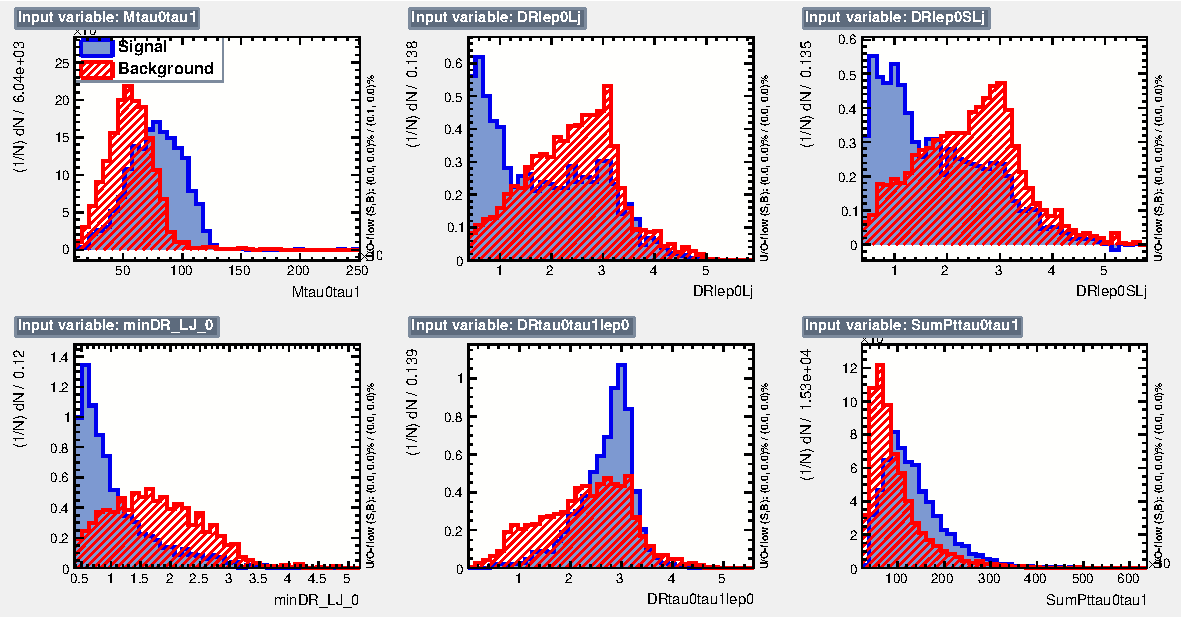
\includegraphics[width=0.8\textwidth, keepaspectratio]{figures/TauChannels/1l2tau/BDT/variables_id_c1.pdf}
    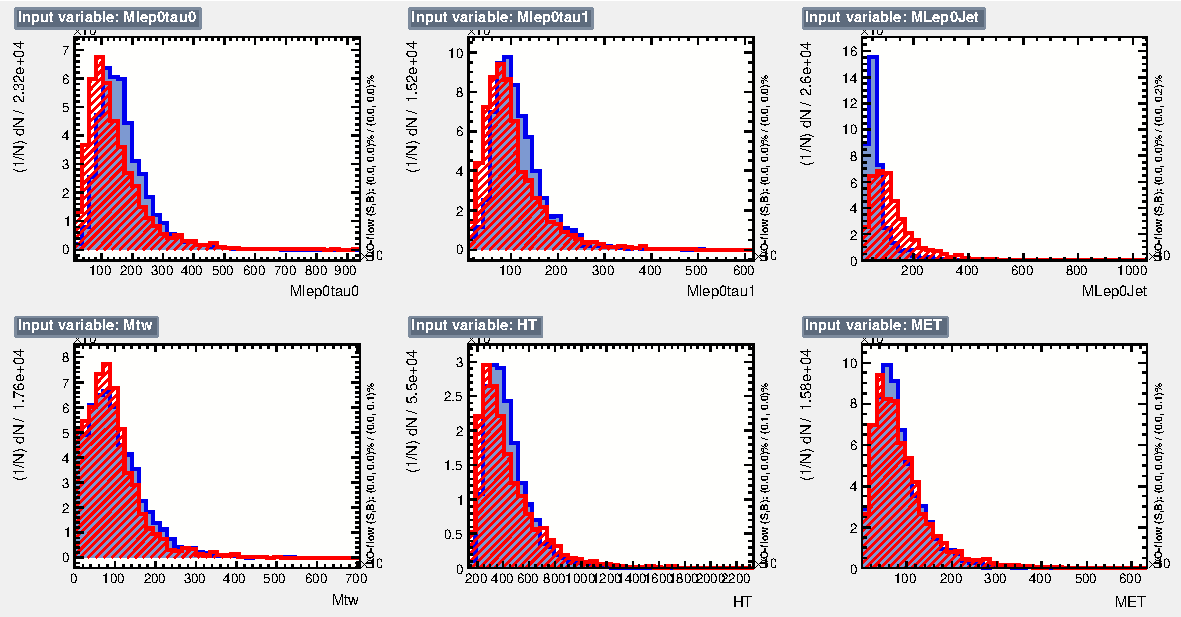
\includegraphics[width=0.8\textwidth, keepaspectratio]{figures/TauChannels/1l2tau/BDT/variables_id_c2.pdf}
  \end{center}
  \caption{\label{fig:BDTinputs_1l2tau} Signal (blue) and background (red) distributions of 12 input variables used in the BDT traning.}
\end{figure}

\begin{figure}[htbp]
  \begin{center}
    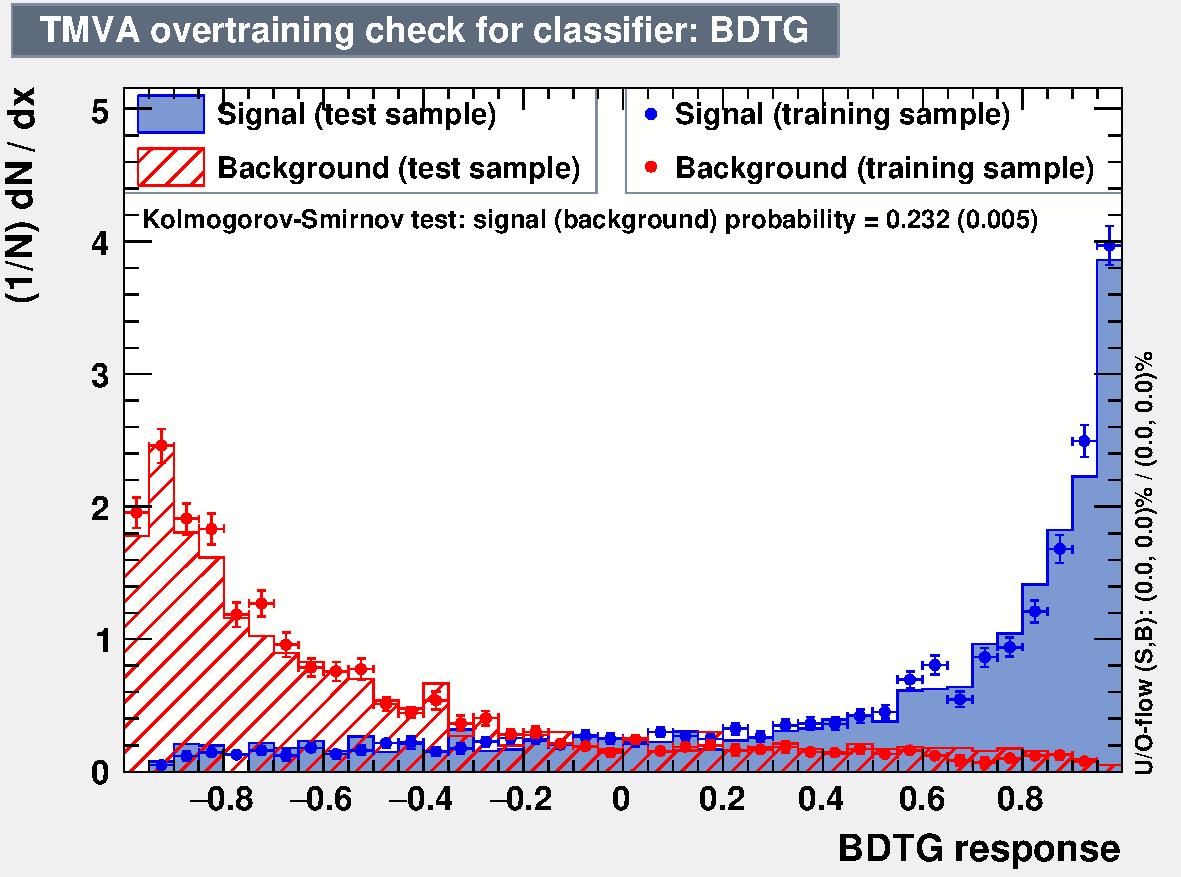
\includegraphics[width=0.49\textwidth, keepaspectratio]{figures/TauChannels/1l2tau/BDT/overtrain_BDTG}
    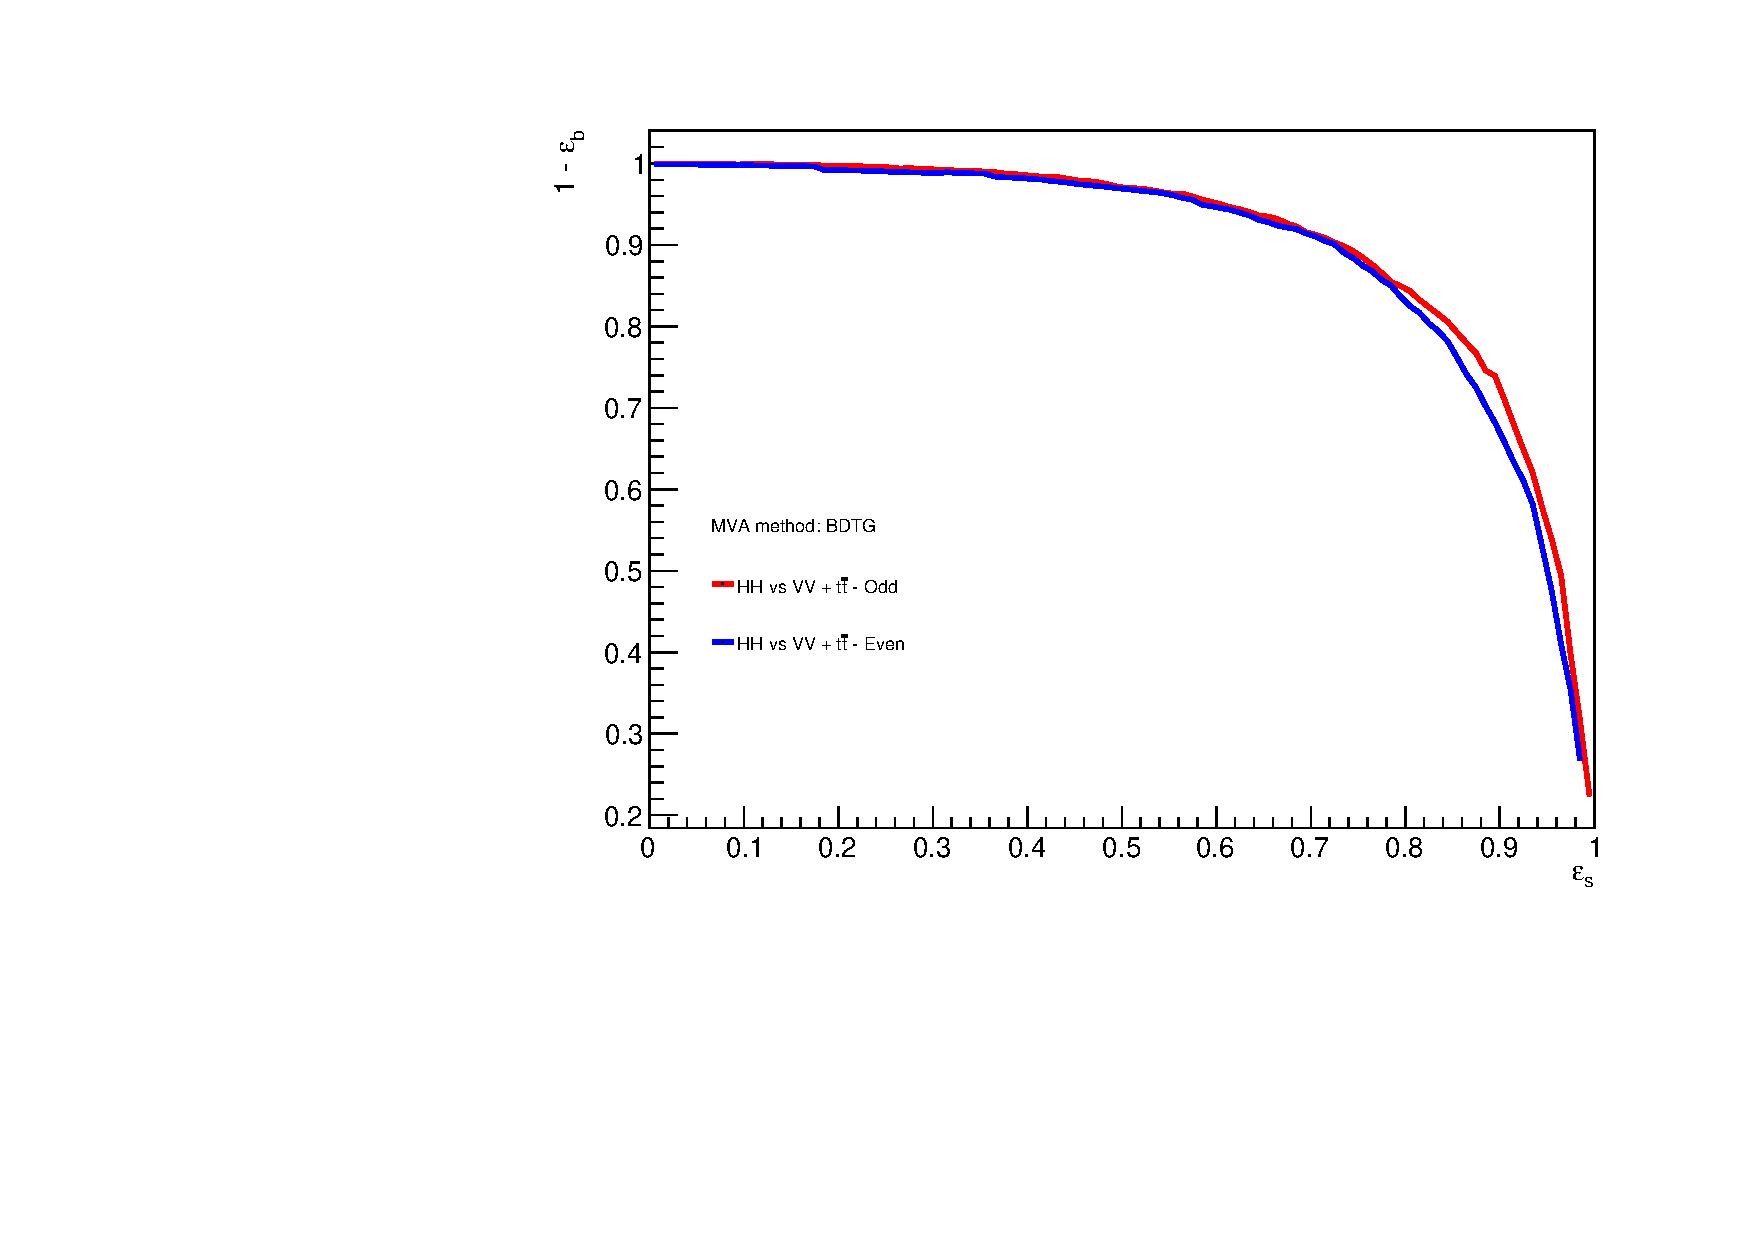
\includegraphics[width=0.5\textwidth, keepaspectratio]{figures/TauChannels/1l2tau/BDT/ROC}
  \end{center}
  \caption{\label{fig:TrainBDT_1l2tau} The BDT distributions for the signal and background obtained during the training and testing (left). The background rejection versus signal efficiency for both BDTs (right).}
\end{figure}

\begin{figure}[htbp]
  \begin{center}
    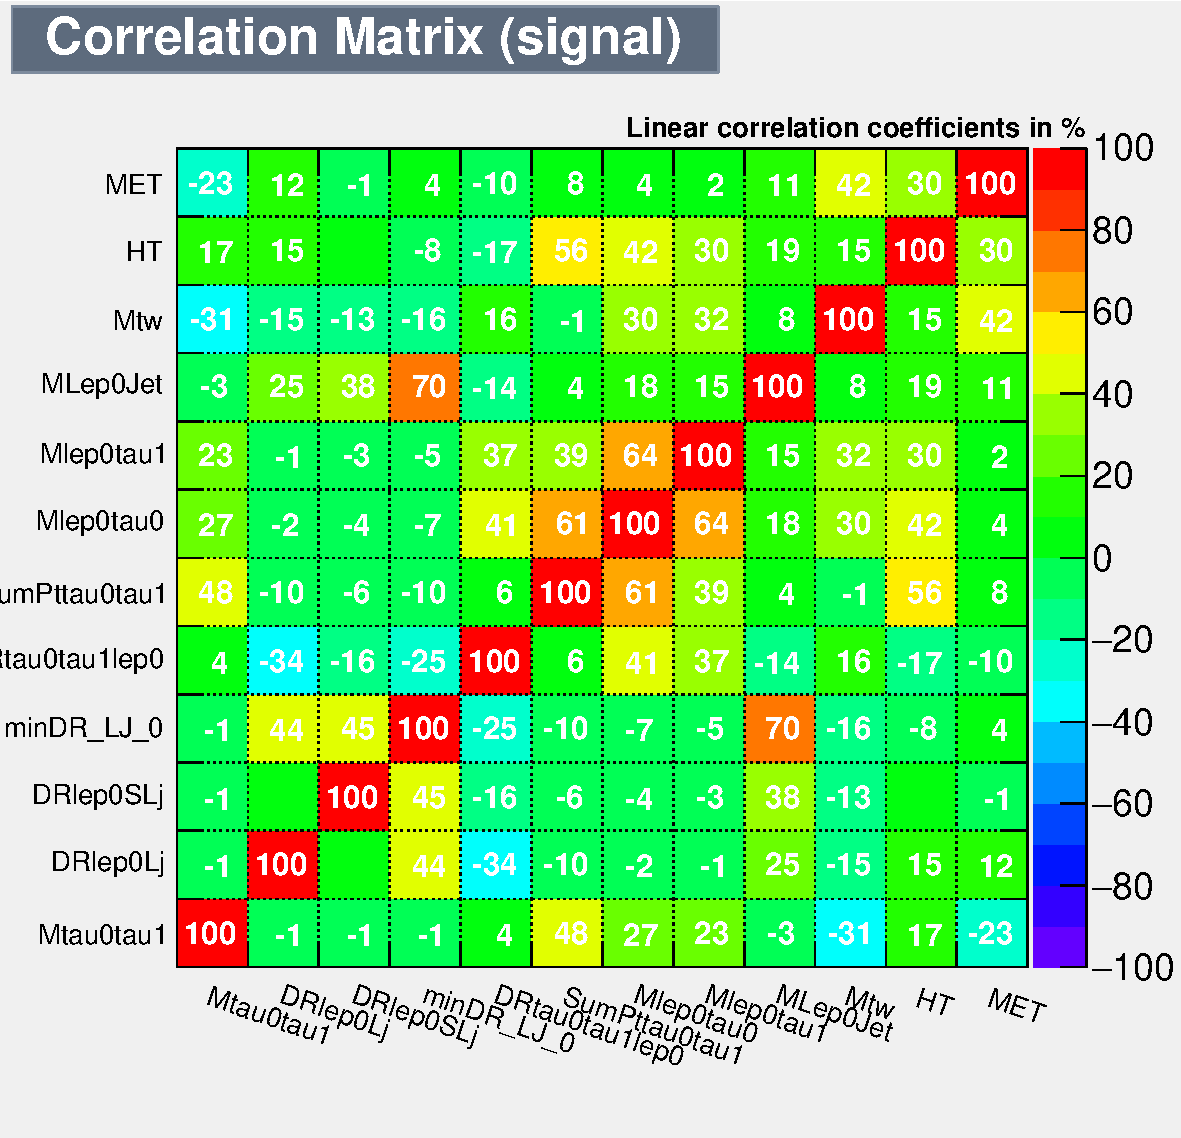
\includegraphics[width=0.49\textwidth, keepaspectratio]{figures/TauChannels/1l2tau/BDT/CorrelationMatrixS}
    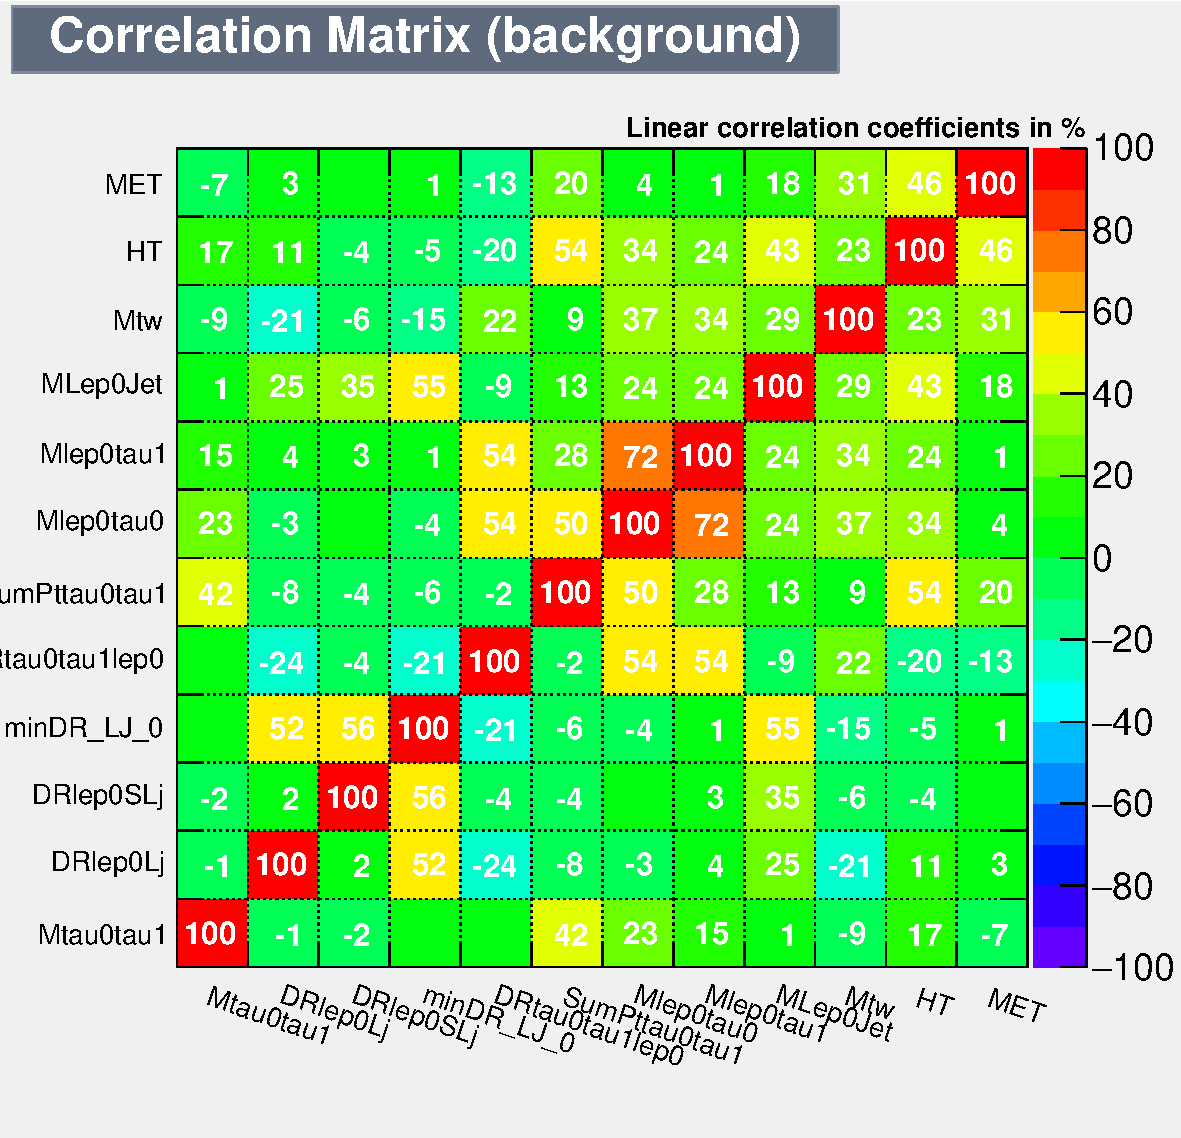
\includegraphics[width=0.49\textwidth, keepaspectratio]{figures/TauChannels/1l2tau/BDT/CorrelationMatrixB}
  \end{center}
  \caption{\label{fig:CorreCoff_1l2tau} Correlation coefficients between the 12 BDT input variables for signal (left) and background (right).}
\end{figure}

\subsubsection{Background estimation}
TBD...

\subsubsection{Systematic uncertainties}
TBD..

\subsubsection{Preliminary results}

Figure~\ref{fig:BDTOutput_1l2tau} shows the pre-fit distribution of the BDT output. A statistical analysis using a profile-likelihood-ratio test statistic is performed using BDT output as a final discriminanat. The signal strangth of non-resonant Standard Model (SM) HH production is defined as the ratio of the signal cross-section to the SM prediction. A preliminary expected limit on the production cross-section for non-resonant hh production is calcualted and is shown in Table~\ref{tab:expeCL_1l2tau}. No systematic uncertainties are included in the profile-likelihood fit.

\begin{figure}[htbp]
  \begin{center}
    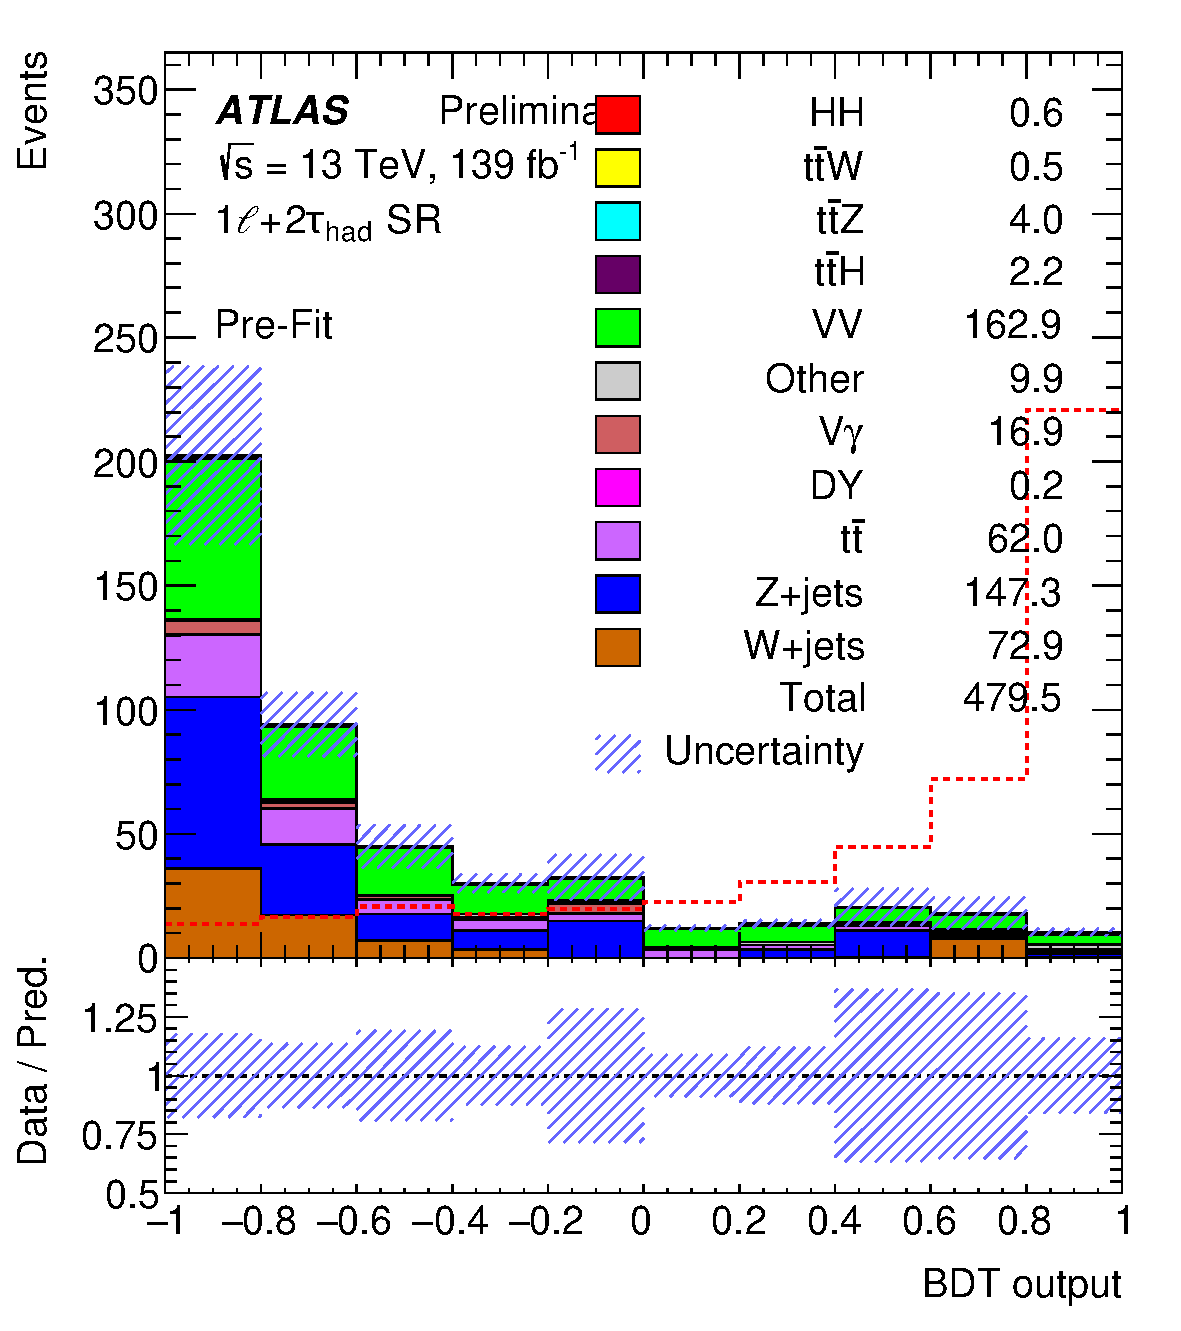
\includegraphics[width=0.49\textwidth, keepaspectratio]{figures/TauChannels/1l2tau/hh_1l2tau_BDT.pdf}
  \end{center}
  \caption{\label{fig:BDTOutput_1l2tau} The BDT distributions expected in the \ltwotau channel. The background pre-fit contributions are shown as filled histograms. The hh signal contribution is scaled and superinposed on the backgrounds.}
\end{figure}

\begin{table}
  \begin{center}
    \begin{tabular}{lccccc}
      \hline
      & & \multicolumn{3}{c}{Expected limit on signal strength}    \\
      \hline
      & Median & +2$\sigma$ & +1$\sigma$ & -1$\sigma$ & -2$\sigma$ \\
      \hline
      \ltwotau     & 32.67 & 75.03 & 49.58 & 23.53 & 17.53\\
      \hline
    \end{tabular}
    \caption{\label{tab:expeCL_1l2tau} Preliminary expected $95\%$ CL exclusion limit on the signal strength.}
  \end{center}
\end{table}
